\section{Préambule : une suite de benchmarks pour OpenMP~4.0, les KASTORS}\label{sec:openmp:kastors}

Cette section présente KASTORS, une suite de benchmarks spécifiquement créée pour rassembler des applications variées utilisant les tâches avec dépendances d'OpenMP.

\subsection{Motivation pour une nouvelle suite de benchmarks}

Le support pour les applications à base de flots de données dans OpenMP est arrivé avec la version 4.0.
Kurzak et al.~\cite{Kurzak2010} ont montré l'intérêt en terme de performances des synchronisations point à point par dépendances de données par rapport aux synchronisations globales.
Cette comparaison a eu lieu entre des applications exprimés dans deux modèles de programmation à base de tâche~: Cilk, où les synchronisations sont explicites, et SMPsS~\cite{BSC2008}, où les synchronisations sont exprimées à l'aide des dépendances de données.

La version~4.0 d'OpenMP est sortie au démarrage de cette thèse, nous n'avions donc pas d'applications de référence utilisant les dépendances de données à travers OpenMP, et nous avons décidé d'introduire une suite de benchmarks - les KASTORS~\cite{Virouleau2014} - spécifiquement orientée vers cette fonctionnalité.
Elle regroupe des applications utilisées dans le HPC~: des algorithmes d'algèbre linéaire dense, un stencil, et une factorisation LU d'une matrice creuse.

Il existe évidemment plusieurs suites de benchmarks à destination des architectures à mémoire partagée~: PARSEC~\cite{Bienia2008}, SPECOMP~\cite{Aslot2001}, Rodinia~\cite{Rodinia2010}, ou encore les NAS~\cite{Bailey1994} sont des suites de benchmarks basées sur des versions antérieures d'OpenMP~(2.0, 3.0), et donc utilisant principalement des boucles parallèles.
La Barcelona OpenMP Task Suite~\cite{Duran2009} (BOTS) propose des applications à base de tâches OpenMP~3.0 afin d'évaluer les implémentations existantes d'OpenMP en fonction de la manière de générer les tâches et de la répartition de la charge de travail.

Certaines applications que nous avons inclues dans KASTORS proviennent de différents benchmarks ou bibliothèques existantes.
Deux applications, SparseLU et Strassen, ont été tirées des BOTS et adaptées pour ne plus utiliser de synchronisations globales.
Trois applications d'algèbre linéaire dense, Cholesky, QR, et LU, ont été tirées des PLASMA~\cite{Kurzak2013}, une bibliothèque développée à ICL/UTK quit met à disposition un grand nombre d'algorithmes d'algèbre linéaire dense, optimisés pour les architectures multi-cœurs.

Nous avions donc assez d'éléments de base pour construire un ensemble d'applications, avec en tête les objectifs suivants~:
\begin{itemize}
  \item Rassembler et proposer une suite d'applications exploitant les dépendances introduites avec OpenMP~4.0~;
  \item Comparer la version utilisant des synchronisations point à point (via des dépendances) à la version utilisant des synchronisations globales. Le but étant de montrer que le support exécutif peut gérer les synchronisations plus finement, et par conséquent améliorer les performances sans changer l'algorithme~;
  \item Permettre d'expérimenter des extensions à OpenMP, dont celles présentées dans les sections~\ref{sec:openmp:langage} et~\ref{sec:openmp:runtime}.
\end{itemize}
%demonstrating the in- terest of task dependencies compared to taskwait-based approaches.

\subsection{Description des applications}

Les sections suivantes décrivent les six applications de la suite : d'où elles viennent et comment nous les avons étendus pour utiliser les dépendances de données.

\subsubsection{Factorisations de Cholesky, QR, et LU}

Ces trois applications ont été extraites des PLASMA, version 2.6~\cite{PLASMA2.6}.
Dans les PLASMA, chaque algorithme est écrit dans différents modèles de programmation~: il existe une version parallélisée statiquement utilisant les threads POSIX, et une autre basée sur QUARK~\cite{YarKhan2011}, un modèle de programmation par flot de données, et utilisant un ordonnancement dynamique.

Les trois algorithmes que nous avons sélectionnés sont les factorisations de Cholesky, QR, et LU, respectivement nommés DPOTRF, DGEQRF, et DGETRF dans les BLAS.
Ils opèrent tous sur des matrices de nombres flottants à double précision (type |double|).

Nous avons adapté l'implémentation originale de PLASMA pour retirer plusieurs niveaux d'encapsulation des fonctions, et ainsi faciliter la lecture et la maintenabilité du code.
Les listings~\ref{lst:kastors:dyn} et~\ref{lst:kastors:dyn-omp} montrent respectivement la version dynamique originale, et les transformations que l'on a faites pour porter le code en OpenMP~4.0.

\begin{lstlisting}[caption=Format de l'algorithme dynamique,label=lst:kastors:dyn]
wrapper_algorithm_call(matrice_description, plasma_specific_args...) {
  // code séquentiel
  for (...) {
    // packing des paramètres
    QUARK_Insert_Task(wrapper_blas_function, packed_parameters);
  }
  // code séquentiel
  for (...) {
    // packing des paramètres
    QUARK_Insert_Task(
        wrapper_another_blas_function,
        packed_parameters);
  }
  // code sequentiel
}
\end{lstlisting}
\begin{lstlisting}[caption=Format de l'algorithme OpenMP,label=lst:kastors:dyn-omp]
algorithm_call(matrice_description) {
    // code séquentiel
    for (...)
#pragma omp task depend(inout:array[...])
        blas_function(...);
    // code séquentiel
    for (...)
#pragma omp task depend(inout:array[...])
        another_blas_function(...);
    // code séquentiel
}
\end{lstlisting}


\subsubsection{Jacobi}

Jacobi est un algorithme itératif pour résoudre un système linéaire d'équations. À chaque itération les différents éléments d'un tableau sont mis à jour en suivant la même formule dépendant des éléments voisins (Stencil).

En pratique cette méthode résout l'équation de Poisson sur le carré unitaire [0,1]x[0,1], qui est divisé en une grille de NxN points espacés régulièrement.
Le noyau de calcul principal est un Stencil à 5 points, en 2 dimensions.
Ce noyau est appliqué successivement jusqu'à ce qu'une convergence soit détectée.

Nous avons implémenté plusieurs versions par blocs de ce noyau~: une reposant sur l'utilisation de boucles parallèles OpenMP (illustrée dans le listing~\ref{lst:kastors:jacobi-for}), une basée sur des synchronisations globales (illustrée dans le listing~\ref{lst:kastors:jacobi-task}), et une basée sur les tâches avec dépendances (illustrée dans le listing~\ref{lst:kastors:jacobi-taskdep}).

\begin{lstlisting}[caption=Boucle itérative principale de Jacobi utilisant des for OpenMP,label=lst:kastors:jacobi-for]
for (it = itold + 1; it <= itnew; it++) {
  // Save the current estimate.
  #pragma omp for collapse(2)
  for (int j = 0; j < ny; j += block_size)
    for (int i = 0; i < nx; i += block_size)
      copy_block(nx, ny, i/block_size, j/block_size, u_, unew_, block_size);

  // Compute a new estimate.
  #pragma omp for collapse(2)
  for (int j = 0; j < ny; j += block_size)
    for (int i = 0; i < nx; i += block_size)
      compute_estimate(i/block_size, j/block_size, u_, unew_, f_,
                       dx, dy, nx, ny, block_size);
}
\end{lstlisting}


\begin{lstlisting}[caption=Boucle itérative principale de Jacobi utilisant des tâches avec synchronisation globales,label=lst:kastors:jacobi-task]
for (it = itold + 1; it <= itnew; it++) {
  // Save the current estimate.
  for (int j = 0; j < ny; j += block_size) {
    for (int i = 0; i < nx; i += block_size) {
      #pragma omp task shared(u_, unew_)
      copy_block(nx, ny, i/block_size, j/block_size, u_, unew_, block_size);
    }
  }

  #pragma omp taskwait

  // Compute a new estimate.
  for (int j = 0; j < ny; j += block_size) {
    for (int i = 0; i < nx; i += block_size) {
      #pragma omp task shared(u_, unew_, f_)
      compute_estimate(i/block_size, j/block_size, u_, unew_, f_,
                       dx, dy, nx, ny, block_size);
    }
  }
  #pragma omp taskwait
}
\end{lstlisting}

\begin{lstlisting}[caption=Boucle itérative principale de Jacobi utilisant des tâches avec dépendances,label=lst:kastors:jacobi-taskdep]
// Calcul des voisins
#define west(i) ((i==0) ? i : i - block_size)
#define east(i) ((i==nx-block_size) ? i : i + block_size)
#define north(j) ((j==ny-block_size) ? j : j + block_size)
#define south(j) ((j==0) ? j : j - block_size)

for (int it = itold + 1; it <= itnew; it++) {
  // Save the current estimate.
  for (int j = 0; j < ny; j += block_size) {
    for (int i = 0; i < nx; i += block_size) {
      #pragma omp task shared(u_, unew_)\
                  depend(in: unew[i][j]) \
                  depend(out: u[i][j])
      copy_block(nx, ny, i/block_size, j/block_size, u_, unew_,
                 block_size);
    }
  }

  // Compute a new estimate.
  for (int j = 0; j < ny; j += block_size) {
    for (int i = 0; i < nx; i += block_size) {
      #pragma omp task shared(u_, unew_)\
                  depend(out: unew[i][j])\
                  depend(in: f[i][j], u[i][j],\
                             u[west(i)][j], u[east(i)][j],\
                             u[i][north(j)], u[i][south(j)])
      compute_estimate(i/block_size, j/block_size, u_, unew_,
                       f_, dx, dy, nx, ny, block_size);
    }
  }
}
\end{lstlisting}

\subsubsection{SparseLU}\label{sec:kastors:sparselu}

Cette application calcule la factorisation LU d'une matrice creuse.
Nous avons modifié l'implémentation originale des BOTS pour ajouter des dépendances de données.
Ces modifications sont décrites dans les listings~\ref{lst:kastors:sparseLU} et~\ref{lst:kastors:sparseLU-deps}.

\begin{parcolumns}[colwidths={1=7.4cm}]{2}
  \colchunk[1]{
\begin{lstlisting}[caption=LU utilisant des tâches indépendantes,label=lst:kastors:sparseLU]
for (k=0; k<NB; k++) {


  lu0(M[k*NB+k]);
  for (j=k+1; j<NB; j++) {


#pragma omp task shared(M)
    fwd(M[k*NB+k], M[k*NB+j]);
  }

  for (i=k+1; i<NB; i++) {


#pragma omp task shared(M)
    bdiv(M[k*NB+k], M[i*NB+k]);
  }
#pragma omp taskwait

  for (i=k+1; i<NB; i++) {
    for (j=k+1; j<NB; j++) {



#pragma omp task shared(M)
      bmod(M[i*NB+k],
           M[k*NB+j],
           M[i*NB+j]);
    }
  }
#pragma omp taskwait
}
\end{lstlisting}
}
\colchunk[2]{
\begin{lstlisting}[caption=LU utilisant des tâches avec dépendances,label=lst:kastors:sparseLU-deps]
for (k=0; k<NB; k++) {
#pragma omp task shared(M)\
    depend(inout: M[k*NB+k])
  lu0(M[k*NB+k]);
  for (j=k+1; j<NB; j++) {
#pragma omp task shared(M)\
    depend(in: M[k*NB+k])\
    depend(inout: M[k*NB+j])
    fwd(M[k*NB+k], M[k*NB+j]);
  }

  for (i=k+1; i<NB; i++) {
#pragma omp task shared(M)\
    depend(in: M[k*NB+k])\
    depend(inout: M[i*NB+k])
    bdiv(M[k*NB+k], M[i*NB+k]);
  }


  for (i=k+1; i<NB; i++) {
    for (j=k+1; j<NB; j++) {
#pragma omp task shared(M)\
        depend(in: M[i*NB+k])\
        depend(in: M[k*NB+j])\
        depend(inout: M[i*NB+j])
      bmod(M[i*NB+k],
           M[k*NB+j],
           M[i*NB+j]);
    }
  }

}
\end{lstlisting}
}
\end{parcolumns}

\subsubsection{Strassen}\label{sec:kastors:strassen}

L'application Strassen utilise des décompositions de matrices pour calculer le produit de grandes matrices denses.
De manière similaire à SparseLU, nous avons modifié l'implémentation des BOTS pour ajouter du parallélisme au niveau des additions dans l'algorithme, et nous avons exprimé des dépendances de données plutôt que d'utiliser une synchronisation à base de |taskwait|.

\subsection{Résumé des performances}

Nous avons évalué l'intérêt des tâches avec dépendances comparées aux tâches indépendantes dans l'article publié à IWOMP2014~\cite{Virouleau2014}.
Les expériences ont été menées sur toutes les applications avec les supports exécutifs de GCC, libGOMP, et de Clang-omp (précurseur du support d'OpenMP dans Clang), libIOMP.
Pour les applications tirée de PLASMA, nous les avons également comparées aux deux versions originales de PLASMA~: statique ou basée sur le modèle par flot de données QUARK.

Les résultats ont montré que l'utilisation des dépendances n'avait jamais d'impact négatif sur les performances.
En particulier pour les applications tirées des PLASMA, nous avons montré que la version OpenMP pouvait être aussi compétitive que la version écrite dans un support exécutif spécifique.
Cela a pu confirmer que les supports exécutifs pouvaient gérer les synchronisations finement, éliminant ainsi les inactivités des threads dues aux |taskwait|, se traduisant du même coup par une amélioration des performances.

\begin{figure}[ht]
  \centering
  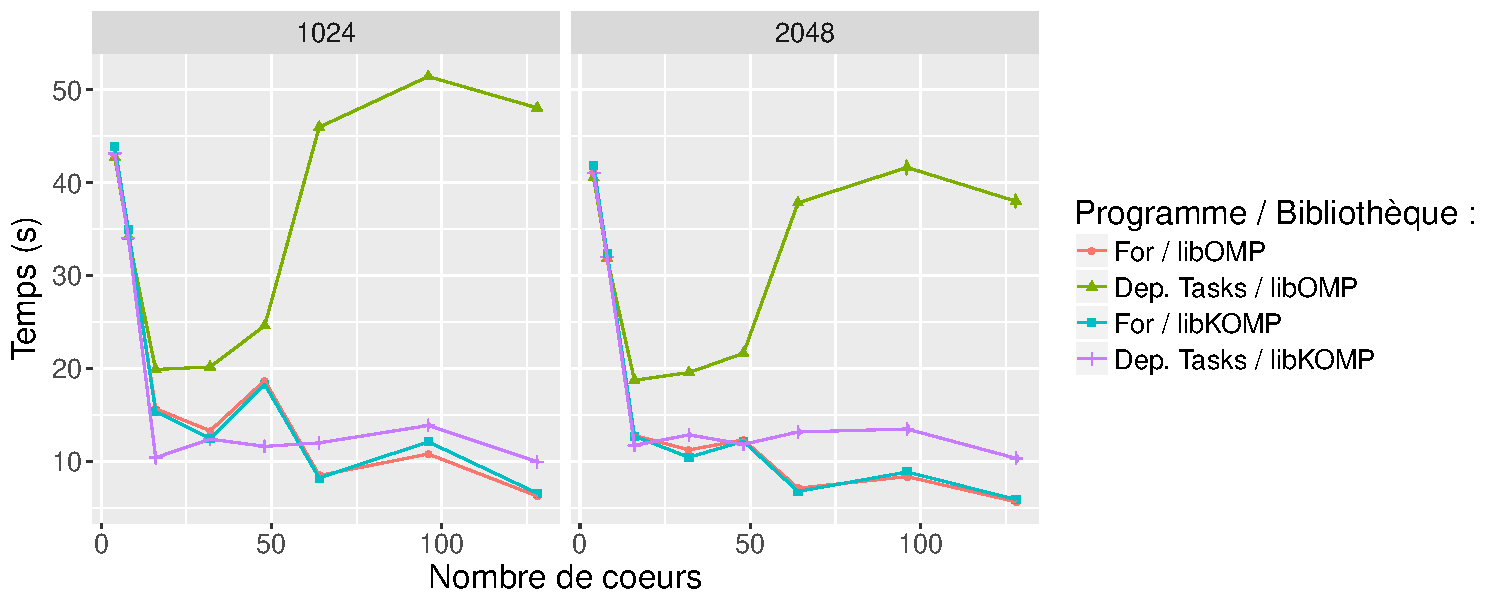
\includegraphics[width=\textwidth]{jacobi_scale_noaff}
  \caption{Comparaison des performances de Jacobi sur idchire, avec une taille de matrice de 49152 et une taille de bloc de 2048}\label{fig:contribs:openmp:kastors:jacobi-motiv}
\end{figure}

D'autres part, certaines de nos expériences ont permis de mettre en évidence d'autres limitations des tâches OpenMP.
La figure~\ref{fig:contribs:openmp:kastors:jacobi-motiv} regroupe une comparaison de l'application de jacobi, en fonction de la version implémentée (à base de boucles ou de tâches avec dépendances) et du support exécutif, effectuée sur idchire.
La scalabilité de l'application en elle-même est limitée, mais il n'y a pas de raison, a priori, qu'il y ait une dégradation de performances de l'application avec l'augmentation du nombre de cœurs.
Jacobi est une application stencil, et chacune des tâches successives (ou groupe d'itérations pour la version à base de boucles) dépend énormément de la réutilisation du cache~: la structure de tâches avec dépendances ne permet pas d'exprimer ce genre de contraintes, lors de l'ordonnancement certaines tâches vont se faire voler et briser la localité des données, introduisant une grosse dégradation des performances.

\subsection{Discussions et perspectives}

Le problème évoqué pour l'application Jacobi vient du fait que l'ordonnanceur n'est pas conscient du lien fort qui existe entre une tâche et ses données, et qu'il permet à plusieurs tâches de s'exécuter loin de leurs données. Une solution possible pourrait être d'attacher les données à des bancs NUMA, et d'exprimer une \emph{contrainte} entre une tâche et un cœur de la machine.

Les résultats de la section~\ref{sec:contribs:apps:cholesky:carton} ont également montrés l'importance de la proximité des données pour les différents noyaux de Cholesky.
Il semble donc très intéressant de pouvoir introduire une clause permettant l'expression d'une \emph{contrainte} entre une tâche et ses données, qui pourrait en fait bénéficier toutes les applications d'algèbre linéaire des KASTORS.

La section suivante aborde ce point, et la section~\ref{sec:contribs:perf_eval} décrit les résultats obtenus à partir des KASTORS étendus avec nos propositions.

